\documentclass[10pt,twocolumn,a4paper]{article}

% ---- IEEE-like formatting ----
\usepackage[top=0.75in, bottom=1in, left=0.625in, right=0.625in]{geometry}
\usepackage{times}
\usepackage[T1]{fontenc}
\usepackage[utf8]{inputenc}
\usepackage{graphicx}
\usepackage{amsmath,amssymb}
\usepackage{booktabs}
\usepackage{tabularx}
\usepackage{multirow}
\usepackage{float}
\usepackage{hyperref}
\usepackage{cite}
\usepackage{caption}
\usepackage{subcaption}
\usepackage{enumitem}
\usepackage{xcolor}
\usepackage{listings}
\usepackage{tikz}
\usetikzlibrary{shapes.geometric, arrows.meta, positioning, fit}
\usepackage{pgfplots}
\pgfplotsset{compat=1.18}
\usepackage{array}
\usepackage{fancyhdr}
\usepackage{titlesec}
\usepackage{url}
\usepackage{balance}

% ---- IEEE-style section formatting ----
\titleformat{\section}{\normalfont\large\bfseries\centering}{\Roman{section}.}{0.5em}{}
\titleformat{\subsection}{\normalfont\normalsize\bfseries\itshape}{\Alph{subsection}.}{0.5em}{}
\titleformat{\subsubsection}{\normalfont\normalsize\itshape}{\arabic{subsubsection})}{0.5em}{}

\titlespacing{\section}{0pt}{12pt plus 2pt minus 2pt}{6pt plus 2pt minus 2pt}
\titlespacing{\subsection}{0pt}{8pt plus 2pt minus 2pt}{4pt plus 2pt minus 2pt}

% ---- Code listing style ----
\lstset{
  basicstyle=\ttfamily\scriptsize,
  breaklines=true,
  frame=single,
  language=Python,
  keywordstyle=\color{blue},
  commentstyle=\color{green!50!black},
  stringstyle=\color{red!70!black},
  showstringspaces=false,
  tabsize=2
}

% ---- Hyperref config ----
\hypersetup{
  colorlinks=true,
  linkcolor=blue!70!black,
  citecolor=blue!70!black,
  urlcolor=blue!70!black
}

\pagestyle{fancy}
\fancyhf{}
\fancyhead[C]{\small TOBB ET\"{U} -- Department of Computer Engineering -- BIL 496 Graduation Project}
\fancyfoot[C]{\thepage}
\renewcommand{\headrulewidth}{0.4pt}

\begin{document}

% ---- Title ----
\title{\LARGE \textbf{FoMAC: Football Match Analysis and Classification}\\[6pt]
\large Final Report}

\author{
\begin{tabular}{ccccc}
Tu\u{g}berk Aksu & Batuhan \c{C}a\u{g}lar & Eray Kaan A\u{g}\"unl\"u & Alperen Tanyel & Yakup \c{C}ak{\i}r\\
\end{tabular}\\[4pt]
\textit{Supervisor: Do\c{c}. Dr. Y\"ucel \c{C}imtay}\\[2pt]
\textit{TOBB University of Economics and Technology, Department of Computer Engineering}\\[2pt]
\textit{Ankara, Turkey}\\[2pt]
April 2026
}

\date{}
\maketitle
\thispagestyle{fancy}

% ================================================================
\begin{abstract}
FoMAC (Football Match Analysis and Classification) is an AI-assisted system that automates the analysis of football matches from single-camera broadcast video footage. The system integrates seven major subsystems into a unified end-to-end pipeline: (1)~YOLOv11-based multi-class object detection for identifying players, referees, and the ball; (2)~advanced multi-object tracking with three candidate implementations including DeepSORT-like, simplified DeepSortTracker, and BoT-SORT-style trackers with Re-Identification (ReID) embeddings and team classification; (3)~a deep learning action spotting module with three model variants (Transformer-based CHATO, RMS-Net-based GEM, and CNN/NetVLAD++ SPOTTING\_V2) for temporal event localization aligned with the SoccerNet-v2 standard; (4)~camera calibration using HRNet-based keypoint and line detection for world-coordinate mapping; (5)~jersey number recognition via both a trained CNN classifier and the Qwen-VL vision-language model; (6)~Turkish commentary generation using Ollama/Gemini LLM backends with XTTS~v2 text-to-speech synthesis using a reference commentator voice; and (7)~a full-stack web dashboard built with Next.js and FastAPI for video upload, pipeline orchestration, progress tracking, and result visualization. This report presents the final architecture, detailed design of each subsystem, implementation specifics, test results, the impact of engineering solutions in economic, environmental, and societal contexts, contemporary issues, and a discussion of all tools, technologies, and resources used throughout the project.
\end{abstract}

% ================================================================
\section{Introduction}

Football is the most popular sport globally, with billions of viewers and a professional ecosystem generating substantial economic activity. Despite this scale, the analysis of match footage remains predominantly a manual endeavor for amateur clubs, lower-league organizations, and independent commentators who lack access to sophisticated broadcast technology. Professional-grade systems such as Opta, StatsBomb, and Hawk-Eye require significant infrastructure investment, creating a barrier for smaller organizations.

The experience of watching and understanding football matches depends heavily on the quality of commentary and analysis provided. Traditional match commentary relies entirely on human commentators who must maintain high performance for extended durations, a physically and mentally demanding task. This dependency introduces several problems: matches without commentary coverage, lack of commentary in specific languages, subjective biases in analysis, and limited accessibility for visually impaired fans who rely on audio descriptions to follow matches.

FoMAC addresses these gaps by providing an end-to-end AI-based analytical pipeline that processes raw football match video through a series of intelligent stages: frame decoding via OpenCV, YOLOv11-based multi-class object detection (player, ball, referee), multi-object tracking via DeepSORT and BoT-SORT algorithms with ReID embeddings, camera calibration for world-coordinate mapping, temporal action spotting using deep learning models, jersey number recognition through vision-language models, natural-language Turkish commentary generation via LLMs with TTS audio synthesis, and presentation through a modern web-based dashboard. The system is designed for accessibility and near-real-time usability, targeting amateur clubs, small broadcasters, and aspiring commentators.

The underlying motivation for this project is to provide football fans with a richer, more interactive match-viewing experience where matches can be analyzed and commented on as if a live commentator were present. The system aims to detect critical events such as goals, cards, fouls, and free kicks while generating emotionally appropriate commentary that adapts to the flow of the match.

The project repository is organized as a collection of major implementation packages across multiple branches, each grounded in specific repository paths. The main branch contains the player detection training pipeline and the web dashboard, while feature branches host tracking prototypes (FoMAC\_Tracking, reid-tracking), multi-class detection, and the commentary engine. This report consolidates findings from all phases of the project.

% ================================================================
\section{Target Audience}

The FoMAC system is designed to serve multiple stakeholder groups, each with distinct needs and use patterns.

\textbf{Football Fans and Enthusiasts:} This group constitutes the largest target audience. Fans who cannot watch matches live or who lack access to detailed analyses can use FoMAC to quickly understand key moments, player performances, and tactical details through the automated commentary system. The commentary-enriched viewing experience aims to make matches more enjoyable and informative, transforming passive viewing into an analytically enriched experience.

\textbf{Sports Analysts and Coaches:} Professional match analysis requires detailed and reliable data on player movements, team formations, and tactical patterns. FoMAC provides automated tracking with world-coordinate mapping, enabling coaches and analysts to extract spatial statistics such as heatmaps, running distances, and ball possession zones. These insights support strategic decision-making, training program optimization, and post-match performance evaluation without requiring expensive commercial analytics platforms.

\textbf{Sports Media and Broadcasters:} Media organizations require timely and comprehensive match coverage. FoMAC enables rapid generation of match summaries, event timelines, and commentary audio, allowing smaller broadcasters and online streaming platforms to produce professional-quality content with significantly reduced reliance on human commentators. This is particularly valuable for covering lower-league matches, women's football, and youth tournaments that receive limited media attention.

\textbf{Visually Impaired Individuals:} A particularly important target group is visually impaired football fans. Through the TTS-powered Turkish commentary system, FoMAC generates detailed audio descriptions of match events, enabling visually impaired users to follow matches through rich spoken narratives. This accessibility feature addresses a significant gap in current sports broadcasting.

\textbf{Independent Content Creators:} Football content creators and aspiring commentators can use FoMAC as a training and production tool. The system allows users to upload match footage and receive AI-generated commentary, which can serve as a reference for developing their own commentary style or as a base for content production.

% ================================================================
\section{Related Work}

The development of AI-powered football commentary and analysis systems has gained significant momentum in recent years, driven by advances in computer vision, natural language processing, and deep learning. This section surveys the most relevant prior work and positions FoMAC within the existing landscape.

\subsection{Object Detection and Tracking in Sports}

Object detection in sports videos has evolved rapidly with the YOLO family of detectors. The original YOLO architecture~\cite{redmon2016yolo} established real-time detection as a feasible paradigm, and subsequent versions have improved accuracy while maintaining speed. In the football domain, several projects have applied YOLO-based detection for player and ball tracking. The ``Detect and Track Players, Referees, and Footballs in a Video Using YOLO''~\cite{football_yolo} project uses pixel segmentation and clustering for player detection with jersey color-based team classification. Similarly, Soccer Video Analytics~\cite{soccer_analytics} by Tryolabs uses YOLO for player detection with team assignment based on visual features.

Multi-object tracking in sports builds upon the DeepSORT~\cite{wojke2017deepsort} and BoT-SORT~\cite{zhang2022botsort} frameworks. DeepSORT introduced appearance-based association through deep features combined with Kalman filtering for motion prediction. BoT-SORT extended this with camera motion compensation and improved association strategies. FoMAC implements both approaches and adds team-aware cost functions and inactive track relinking mechanisms tailored to the football domain, where players frequently occlude each other and camera angles change during replays.

\subsection{Action Spotting and Event Detection}

Temporal action localization in sports videos has been formalized through the SoccerNet benchmark~\cite{soccernet}. The SoccerNet-v2 challenge defines 17 action classes and provides standardized evaluation protocols. The Football Analysis~\cite{football_analysis} project addresses similar event detection tasks focusing on goals, fouls, and offsides. FoMAC extends this scope to include a broader range of events using three distinct architectures (Transformer-based, RMS-Net with Gaussian encoding, and CNN/NetVLAD++ hybrid), enabling comparative evaluation and ensemble potential.

The NetVLAD architecture~\cite{arandjelovic2016netvlad}, originally designed for visual place recognition, has been adapted for temporal feature aggregation in sports video analysis. FoMAC's SPOTTING\_V2 model employs a dual NetVLAD++ approach with separate past/future pooling, providing asymmetric temporal context that is particularly effective for anticipating and confirming event boundaries.

\subsection{AI-Generated Sports Commentary}

The concept of AI-generated football commentary has been explored in several projects. The ``AI Generating Real-Time Football Commentary''~\cite{football_ai_commentary} project demonstrates automated commentary generation, though primarily in English. The key challenge in this domain is generating commentary that is not only factually accurate but also emotionally engaging and linguistically natural.

FoMAC differentiates itself from existing commentary systems in several important ways. First, it generates commentary specifically in Turkish, addressing a significant gap for the Turkish football community. Second, it employs voice cloning through XTTS v2 with a reference commentator voice, producing output that sounds like a specific professional commentator rather than generic TTS. Third, the commentary engine incorporates sophisticated prompt engineering with style rotation, tactical vocabulary, and dynamic adaptation to match intensity---features that go beyond simple event narration.

\subsection{Camera Calibration for Sports Analytics}

Camera calibration for sports field mapping has been addressed through various approaches. The SoccerNet camera calibration challenge provides benchmarks for pitch-to-image alignment. HRNet~\cite{sun2019hrnet} has proven effective for keypoint detection in this context. FoMAC's calibration pipeline uses dual HRNet models (58 keypoints + 24 lines) with homography estimation and PnP solvers, enabling per-frame or sequence-based calibration with temporal interpolation. This approach handles camera angle changes gracefully, which is a common challenge in broadcast footage where camera angles change frequently during replays and different shot types.

\subsection{Positioning of FoMAC}

While individual components of FoMAC (detection, tracking, event spotting, commentary) have been explored separately in the literature, FoMAC is distinguished by its end-to-end integration of all these components into a single, unified pipeline. Most existing projects address only one or two aspects---detection and tracking without commentary, or commentary without calibrated spatial analysis. FoMAC combines all seven subsystems (detection, tracking, ReID with team classification, calibration, action spotting, jersey recognition, and commentary with TTS) into a cohesive system accessible through a web dashboard, targeting deployment on consumer hardware rather than requiring cloud infrastructure.

% ================================================================
\section{Unique Contributions}

While FoMAC builds upon established computer vision and NLP techniques, several aspects distinguish it from prior work and similar projects.

\textbf{Comprehensive Event Coverage:} Unlike projects that focus solely on major events (goals, cards), FoMAC's action spotting module detects 17 distinct event types aligned with the SoccerNet-v2 standard, including corners, throw-ins, free kicks, clearances, saves, and ball-out-of-play events. This comprehensive coverage enables richer, more detailed commentary that captures the full narrative of a match rather than just highlight moments.

\textbf{Dynamic AI Commentary with Emotional Adaptation:} FoMAC's commentary engine goes beyond simple event narration. The system uses five rotating commentary styles (high-tempo, tactical, wing-focused, midfield pressure, penalty area threat) and dynamically adapts to match intensity based on spatial analysis from calibration data. The prohibition of uncertainty expressions and enforcement of word budgets ensures confident, broadcast-quality output.

\textbf{Camera Angle Sensitivity:} Many existing projects do not adequately handle camera angle changes, which are frequent in broadcast footage. FoMAC's BoT-SORT tracker includes histogram-based scene change detection that triggers tracker reset or soft reset during camera transitions and replays, maintaining tracking integrity across shot boundaries. The calibration module provides per-frame or sequence-based calibration with temporal interpolation for smooth world-coordinate mapping.

\textbf{Turkish Language Focus with Voice Cloning:} FoMAC specifically targets Turkish-language commentary, addressing a gap in the sports AI landscape. The XTTS v2 integration with reference speaker conditioning produces commentary that mimics a specific professional commentator's voice, including Turkish phonological normalization (e.g., handling the ``gol'' $\rightarrow$ ``g\^{o}l'' pronunciation for correct articulation).

\textbf{Multi-Architecture Comparison:} Rather than committing to a single model for tracking and action spotting, FoMAC implements multiple architectures for comparative evaluation: three tracker variants (DeepSORT, simplified DeepSort, BoT-SORT with team fusion) and three action spotting models (Transformer, RMS-Net/GEM, CNN/NetVLAD++). This enables runtime selection based on accuracy/speed trade-offs and provides a rich experimental framework.

\textbf{Consumer Hardware Deployment:} The system is designed for deployment on consumer-grade hardware (RTX 3060-class GPU, Intel i5 CPU), making it accessible to amateur clubs, small broadcasters, and individual users. The quantized Qwen-VL model (Q4\_K\_M GGUF) and lightweight YOLOv11n backbone demonstrate the viability of running complex multi-stage AI pipelines without enterprise infrastructure.

% ================================================================
\section{System Architecture and Design}

\subsection{High-Level Pipeline Architecture}

The FoMAC system implements a multi-stage pipeline architecture as illustrated in Fig.~\ref{fig:pipeline}. The pipeline processes video input through the following stages sequentially, orchestrated by the \texttt{FullPipelineConfig} dataclass that encapsulates over 50 configurable parameters.

\begin{figure}[H]
\centering
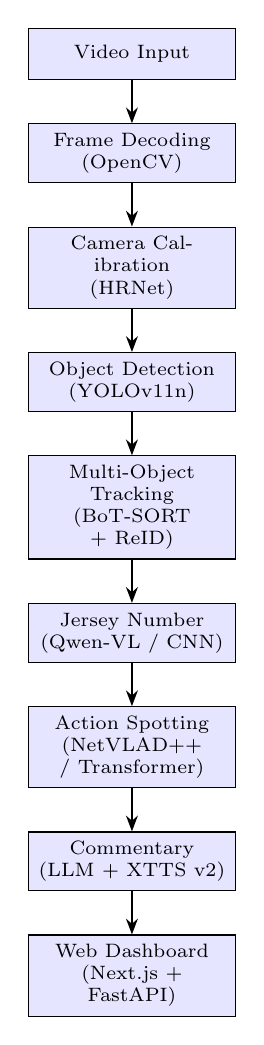
\begin{tikzpicture}[
  node distance=0.55cm,
  block/.style={rectangle, draw, fill=blue!10, text width=2.4cm, text centered, minimum height=0.65cm, font=\scriptsize},
  arrow/.style={-{Stealth[length=2mm]}, thick}
]
\node[block] (input) {Video Input};
\node[block, below=of input] (decode) {Frame Decoding \\ (OpenCV)};
\node[block, below=of decode] (calib) {Camera Calibration \\ (HRNet)};
\node[block, below=of calib] (detect) {Object Detection \\ (YOLOv11n)};
\node[block, below=of detect] (track) {Multi-Object Tracking \\ (BoT-SORT + ReID)};
\node[block, below=of track] (jersey) {Jersey Number \\ (Qwen-VL / CNN)};
\node[block, below=of jersey] (event) {Action Spotting \\ (NetVLAD++ / Transformer)};
\node[block, below=of event] (comment) {Commentary \\ (LLM + XTTS v2)};
\node[block, below=of comment] (web) {Web Dashboard \\ (Next.js + FastAPI)};

\draw[arrow] (input) -- (decode);
\draw[arrow] (decode) -- (calib);
\draw[arrow] (calib) -- (detect);
\draw[arrow] (detect) -- (track);
\draw[arrow] (track) -- (jersey);
\draw[arrow] (jersey) -- (event);
\draw[arrow] (event) -- (comment);
\draw[arrow] (comment) -- (web);
\end{tikzpicture}
\caption{FoMAC end-to-end processing pipeline.}
\label{fig:pipeline}
\end{figure}

\subsection{Detection and Training Package}

The detection subsystem is built on the Ultralytics YOLOv11n architecture, chosen for its balance between inference speed and detection accuracy. The system supports two detection modes.

\subsubsection{Single-Class Player Detection}
The primary production-ready pipeline is located in \texttt{model-training/player-detection/}. The orchestrator class \texttt{YOLOTrainingPipeline} in \texttt{main.py} manages the full lifecycle including dataset extraction, training, evaluation, and prediction via YAML-driven configuration files. It parses command-line arguments for hyperparameter overrides and supports five pipeline modes: extraction only, training only, full pipeline, evaluation, and prediction.

The configuration subsystem uses four YAML files: \texttt{paths.yaml} defines workspace roots, SoccerNet paths, dataset roots, model roots, report roots, and file patterns (e.g., \texttt{\{half\}\_720p.mkv} for video, \texttt{\{half\}\_player\_boundingbox\_maskrcnn.json} for annotations); \texttt{extraction.yaml} defines detection start time (\texttt{det\_start\_sec}), detection FPS (\texttt{det\_fps}), frame shift compensation, and class names (currently only ``player'' with class\_id hardcoded to 0); \texttt{device.yaml} defines device selection priority (CUDA $\rightarrow$ DirectML via torch\_directml $\rightarrow$ CPU); and \texttt{yolo\_params.yaml} defines training hyperparameters.

The \texttt{DatasetExtractor} class (\texttt{modules/dataset\_extractor.py}) loads SoccerNet-style JSON detection files, aligns timestamps to video frames handling detection start time, detection FPS, actual video FPS, and frame shift compensation, converts bounding boxes to YOLO format, and generates label files. The \texttt{YOLOTrainer} class (\texttt{modules/trainer.py}) wraps \texttt{ultralytics.YOLO}, builds training config dictionaries from YAML, and exposes \texttt{train()}, \texttt{evaluate()}, and \texttt{predict()} methods. The \texttt{DeviceManager} class (\texttt{modules/device\_manager.py}) implements automatic hardware detection with the priority cascade: CUDA $\rightarrow$ DirectML $\rightarrow$ CPU.

The training pipeline also includes a report generation system (\texttt{reports/report\_generator.py}) that automatically produces Excel and HTML performance reports with per-class precision, recall, and mAP metrics.

\subsubsection{Multi-Class Detection (Ball Detection)}
An extended pipeline in \texttt{model-training/ball-detection/yolo/} handles three classes---Player (86\%), Ball (5.7\%), and Referee (8.4\%)---using transfer learning from the base player detection model. The dataset comprises approximately 11,673 annotated images configured via \texttt{ballDataset/data.yaml}. Ball detection remains technically challenging due to the small pixel footprint in wide-angle footage and motion blur during fast passes.

This pipeline includes visualization utilities (\texttt{visualize\_labels.py}, \texttt{visualize\_specific\_class.py}) for dataset quality assurance, video prediction scripts (\texttt{video\_prediction.py}), and examples (\texttt{examples.py}) for quick testing. The detection model trained here (\texttt{best.pt}) serves as the primary detector for the entire downstream tracking and analysis pipeline.

\subsection{Multi-Object Tracking Package}

Tracking is architecturally the most complex subsystem in FoMAC, with three candidate implementations explored and evaluated during development.

\subsubsection{Candidate A: DeepSORT-like Tracker (FoMAC\_Tracking Branch)}
Located in \texttt{model-training/FoMAC\_Tracking/src/tracker/}, this implementation is a modular DeepSORT variant. The core \texttt{Tracker} class uses a two-stage association strategy: the first stage employs cosine distance on ReID embeddings with Kalman filter gating on confirmed tracks, and the second stage uses IoU-based fallback matching for unconfirmed or newly appearing tracks. The Hungarian algorithm (\texttt{linear\_sum\_assignment}) resolves assignment. Track states transition through tentative $\rightarrow$ confirmed $\rightarrow$ deleted (after \texttt{max\_age} frames without matches).

The \texttt{Track} class (\texttt{track.py}) maintains state vectors including mean, covariance, feature embedding, hit count, age, and confirmation status, with methods \texttt{update()}, \texttt{predict()}, \texttt{to\_xyxy()}, and \texttt{to\_tlbr()}. The \texttt{KalmanFilter} (\texttt{kalman\_filter.py}) uses a 7-dimensional state vector $[c_x, c_y, \text{aspect\_ratio}, h, v_x, v_y, v_w]$ for motion prediction. The matching module (\texttt{matching.py}) implements both cosine distance and IoU-based matching with the Hungarian algorithm.

This branch also includes a complete orchestration entry point (\texttt{main.py}) that coordinates video decoding, YOLO detection (\texttt{YOLODetector} class), ReID extraction, tracking, event spotting, and visualization with video recording capabilities.

\subsubsection{Candidate B: Simplified DeepSortTracker}
Located in \texttt{model-training/trackers/deepsort\_tracker.py}, this is a self-contained lightweight prototype using greedy matching with optional feature-based matching and geometry-based similarity fallback. It implements the same conceptual pipeline but with reduced complexity, suitable for rapid prototyping and evaluation.

\subsubsection{Candidate C: BoT-SORT-style Tracker (ReID + Team Fusion)}
The most advanced implementation, located in \texttt{model-training/tracking-reid-osnet/}, features a comprehensive multi-stage association strategy. The \texttt{BoTSORTTeamReIDTracker} class combines IoU + appearance + team penalty fusion with configurable weights: $w_{\text{iou}} = 0.6$, $w_{\text{app}} = 0.35$, $w_{\text{team}} = 0.05$. Key features include:

\begin{itemize}[noitemsep,topsep=0pt]
  \item \textbf{Two-stage association:} Primary matching using IoU + appearance + team similarity, followed by IoU-only recovery for unmatched detections.
  \item \textbf{Inactive track relinking:} An inactive pool maintains tracks for up to 900 frames, enabling re-identification after prolonged occlusion. The relinking mechanism uses appearance similarity (cosine distance) with configurable thresholds.
  \item \textbf{Team classification:} The \texttt{AutoLabEmbedder} extracts Lab color space features from torso crops (with green pitch masking), and \texttt{AutomaticTeamClusterer} performs K-means clustering to assign team IDs automatically.
  \item \textbf{Special track handling:} Goalkeeper tracks (IDs $\geq$ 800,000,000) and referee tracks (IDs $\geq$ 900,000,000) are handled separately with dedicated logic.
  \item \textbf{Scene change detection:} Histogram-based cut detection triggers tracker reset or soft reset during camera angle changes and replay sequences.
  \item \textbf{Multi-embedding memory gallery:} Each track maintains a gallery of appearance embeddings for robust re-identification.
  \item \textbf{Ball tracking:} Separate IoU-only single-track pipeline for ball detection (class\_id = 1).
\end{itemize}

The tracker is configured via \texttt{config.yaml} with extensive parameters: gating thresholds (iou\_gate = 0.05, app\_gate = 0.2), max\_age = 90 frames, min\_hits = 3, and reacquisition settings. The output schema produces CSV files with columns: \texttt{frame\_id, track\_id, cls\_id, conf, x1, y1, x2, y2, team\_id, relinked, relink\_source\_id, relink\_sim, relink\_inactive\_age, assoc\_stage, assoc\_iou, assoc\_app\_sim, assoc\_osnet\_sim}---the richest structured output in the repository.

\subsection{Re-Identification (ReID) Package}

ReID generates appearance embeddings for detected players, consumed by the tracking modules. Two distinct implementations exist, each tightly coupled to its corresponding tracker.

\subsubsection{OSNet-based ReID (FoMAC\_Tracking Branch)}
The \texttt{ReIDExtractor} class in \texttt{FoMAC\_Tracking/src/reid/reid\_extractor.py} uses the torchreid library with the OSNet\_x1\_0 backbone. It applies torchvision transforms (Resize to $[256, 128]$, ToTensor, ImageNet normalization) and produces 512-dimensional L2-normalized embeddings per detection. Dependencies include torch, torchvision, torchreid, and numpy.

\subsubsection{ConvNeXt-Large/OSNet Hybrid ReID (BoT-SORT Branch)}
The reid-tracking branch employs a more advanced \texttt{ConvNeXtLargeReID} (nn.Module) extractor that can load ConvNeXt-Large checkpoints, TorchScript models, or fall back to torchreid OSNet. This design supports both the SoccerNet ReID pretrained weights and imagenet-pretrained OSNet, integrated directly into the BoT-SORT multi-stage association logic.

\subsection{Event (Action) Spotting Package}

The event spotting module has been developed with three distinct model architectures, all designed for temporal action localization aligned with the SoccerNet-v2 standard supporting 17 action classes (Goal, Foul, Shot, Corner, Throw-in, Penalty, Offside, Yellow Card, Red Card, Substitution, Clearance, Save, Ball Out of Play, Direct Free-kick, Indirect Free-kick, Kick-off).

\subsubsection{CHATO: Transformer-based Action Spotter}
Located in \texttt{model-training/action\_spotting/chato/}, the \texttt{ActionSpottingTransformerNet} uses an input projection layer ($8576 \rightarrow 512$ dimensions) followed by a 2-layer \texttt{TransformerEncoder} with multi-head attention. The model predicts action classes based on the center frame of the temporal window, processing input tensors of shape $(B, T, 8576)$ and producing output of shape $(B, 18)$ (17 actions + background). Training uses Adam optimizer with $lr = 10^{-4}$ and batch size 8.

\subsubsection{GEM: RMS-Net with Gaussian Encoding}
Located in \texttt{model-training/action\_spotting/gem/}, the \texttt{RMSNet} class employs a 1D-CNN backbone with Conv1d projections, GroupNorm (suited for low-batch training), and 3 residual blocks with ReLU and dropout (0.25). The key innovation is Gaussian labeling ($\sigma = 2.0$) that spreads annotation labels temporally, enabling per-frame supervision. The configuration uses a window size of 20 seconds (40 frames at 2.0 FPS). Training employs Automatic Mixed Precision (AMP) with \texttt{GradScaler} and weighted positive examples via \texttt{calculate\_weights\_sqrt()}, handling class imbalance (Goal receives higher weight, Throw-in lower). Batch size is 8, learning rate $10^{-4}$, over 50 epochs.

\subsubsection{SPOTTING\_V2: CNN/NetVLAD++ Hybrid}
Located in \texttt{model-training/action\_spotting/spotting\_v2/}, this is the most advanced action spotting model. The \texttt{CNNActionSpotter} architecture combines:

\begin{itemize}[noitemsep,topsep=0pt]
  \item \textbf{Input projection:} Linear layer ($8576 \rightarrow 512$)
  \item \textbf{1D-CNN backbone:} Conv1d layers with BatchNorm for temporal pattern capture
  \item \textbf{NetVLAD++ dual pooling:} Two independent NetVLAD layers (\texttt{netvlad\_past} and \texttt{netvlad\_future}) with $K=64$ learnable cluster centers each, splitting the temporal window into ``Past'' and ``Future'' segments for asymmetric temporal understanding. NetVLAD output dimension: $2 \times 64 \times 512 = 65{,}536$
  \item \textbf{Classification head:} Linear$(65536) \rightarrow 512 \rightarrow (N_{\text{classes}} + 1)$
  \item \textbf{Regression head:} Separate MLP for temporal offset prediction
\end{itemize}

The model uses a hybrid loss combining Focal Loss (to address background vs.\ 17-class imbalance) and MSE Regression Loss for temporal offset refinement. Performance is measured via mAP. The configuration supports both Baidu ($8576$ dims) and ResNet ($512$ dims) features with masking probability 0.5 for data augmentation. An alternative \texttt{ActionTransformer} model is also available for comparison.

The \texttt{SoccerNetDataset} class handles feature loading, temporal jittering, and RMS-Net-inspired masking. The \texttt{TrainingPipeline} manages the optimization loop with per-class mAP evaluation and checkpoint persistence.

Additionally, there is a heuristic-based \texttt{EventSpotter} (\texttt{model-training/spotters/event\_spotter.py}) that operates on tracking output directly. It uses a deque-based temporal window (5 frames) to calculate ball speed for shot detection (threshold: 20 px/s with smoothing factor 0.7) and player acceleration for sprint detection (threshold: 100 px/s\textsuperscript{2}), with duplicate prevention through frame buffering.

\subsection{Camera Calibration Module}

The calibration pipeline (\texttt{model-training/calibration/}) performs camera-to-pitch alignment using High-Resolution Networks (HRNet) for keypoint and line detection. Two HRNet models are employed:

\begin{itemize}[noitemsep,topsep=0pt]
  \item \textbf{Keypoints model:} Detects 58 joints corresponding to pitch markings and boundaries on $960 \times 540$ input images using a multi-stage architecture (BOTTLENECK $\rightarrow$ BASIC blocks) with channel progression $[48, 96, 192, 384]$.
  \item \textbf{Lines model:} Detects 24 joints corresponding to field lines using the same HRNet architecture with a separate weight file.
\end{itemize}

The calibration uses heatmap-based keypoint extraction from \texttt{nbjw\_calib/utils/utils\_heatmap.py}, geometric transformations via homography estimation and PnP (Perspective-n-Point) solvers from \texttt{utils\_geometry.py}, and the SoccerNet baseline camera/pitch modules. The \texttt{FramebyFrameCalibration} class provides per-frame calibration, while sequence-based calibration (\texttt{utils\_calib\_seq.py}) provides temporal interpolation for smooth world-coordinate mapping.

The calibration runs as a subprocess via \texttt{run\_pipeline\_calibration.py}, producing a minimap video (\texttt{out\_map}), events JSON (\texttt{out\_events}), and optionally frame-level JSONL data with world-space player and ball positions. The pipeline supports configurable frame windows (\texttt{yolo\_frame\_window}), ball-priority selection modes, and linear interpolation for missing frames.

\subsection{Jersey Number Recognition}

FoMAC implements two approaches for jersey number recognition:

\subsubsection{CNN-based Classifier}
Located in \texttt{model-training/jersey\_number\_recognition/}, this module provides a traditional deep learning approach. The model (\texttt{model.py}) supports multiple backbones (ResNet18, ResNet34, ResNet50, MobileNetV2) with ImageNet pretraining and a final FC layer mapping to jersey number classes. The training pipeline (\texttt{train.py}) uses Albumentations for augmentation (rotation, perspective, erasing), 80/20 train/val split, and generates confusion matrices and per-class AP metrics. The dataset loader handles class imbalance with a maximum of 500 samples per class. A label mapping file (\texttt{label\_mapping.json}) maps 44 class indices to actual jersey numbers (0--93, with gaps).

\subsubsection{Qwen-VL Vision-Language Model}
The production pipeline uses Qwen3VL-8B-Instruct (Q4\_K\_M GGUF quantized) running as a containerized inference service via llama.cpp. The system crops player bounding boxes from tracked frames and queries the vision-language model with a structured prompt requesting digit-only output. Configuration includes maximum tracks per frame (\texttt{jersey\_frame\_topk} = 5), minimum detection confidence (0.55), minimum bounding box area ($40 \times 40$ pixels), minimum frame gap between queries (20 frames), optional visibility filtering (\texttt{jersey\_vis\_filter}), and confidence-based merging (\texttt{jersey\_merge\_same\_number} with \texttt{jersey\_merge\_min\_confidence} = 0.60).

The pipeline manages GPU resources by optionally stopping the Qwen-VL container before commentary generation (\texttt{qwen\_vl\_stop\_before\_commentary}) to free VRAM.

\subsection{Commentary Generation Package}

The commentary engine generates natural-language Turkish commentary for detected match events using a sophisticated multi-stage approach.

\subsubsection{LLM Text Generation}
The system supports two LLM backends: Ollama (local, default model: \texttt{qwen3.5:9b}) and OpenAI-compatible APIs (llama.cpp, vLLM). The prompt engineering is highly domain-specific, instructing the model to act as a Turkish football commentator with rules for: only Turkish output, JSON format compliance, sentence/word budgets calibrated to segment duration, prohibition of uncertainty expressions (``belki'', ``muhtemelen'', ``olabilir''), and incorporation of tactical football language (wing play, center connections, penalty area proximity, defensive transitions).

The \texttt{\_build\_commentary\_item\_prompt()} function generates per-window prompts incorporating match state data from calibration frames (ball world coordinates, lane/band labels, pressure levels), recent commentary history (to avoid repetition), and style variation (5 rotating commentary styles: high-tempo, tactical, wing-focused, midfield pressure, penalty area threat).

The commentary pipeline includes: \texttt{\_sanitize\_commentary\_text()} for filtering banned phrases, \texttt{\_trim\_commentary\_text()} for enforcing sentence/word budgets, \texttt{\_is\_repetitive\_commentary()} for duplicate detection, and \texttt{\_fallback\_commentary\_text()} for generating rule-based commentary when LLM fails.

\subsubsection{TTS Audio Synthesis}
The \texttt{CommentaryEngine} class (\texttt{web/backend/commentary\_engine.py}) synthesizes Turkish audio using Coqui XTTS v2 with a reference speaker WAV file (\texttt{ertem\_sener.wav}). Key implementation details include:

\begin{itemize}[noitemsep,topsep=0pt]
  \item \textbf{Speaker conditioning:} Pre-computed GPT conditioning latents and speaker embeddings cached from the reference WAV (\texttt{gpt\_cond\_len=12, gpt\_cond\_chunk\_len=4, max\_ref\_length=10}).
  \item \textbf{Turkish text normalization:} Collapsing double punctuation (causes long noisy output), converting trailing periods to exclamation marks (cleaner cutoff), and replacing ``gol'' with ``g\^{o}l'' to nudge XTTS toward ince L (front/light L) articulation instead of the default kal{\i}n L (dark/back L) due to Turkish phonological rules.
  \item \textbf{Sentence splitting:} Text split on sentence boundaries for better prosody, with 50ms silence gaps between chunks.
  \item \textbf{Synthesis parameters:} temperature=0.65, repetition\_penalty=5.0, top\_k=50, top\_p=0.85, speed=1.0, sample rate 24000~Hz.
  \item \textbf{Audio validation:} Minimum file size check (2048 bytes) to reject corrupted outputs.
  \item \textbf{Platform compatibility:} Patching XTTS \texttt{load\_audio()} to use soundfile+librosa instead of torchaudio/torchcodec (Windows TorchCodec DLL issues).
\end{itemize}

Commentary audio clips are mixed into the overlay video using FFmpeg with precise timestamping, producing the final output MP4.

\subsection{Web Dashboard}

The web interface implements a modern full-stack architecture.

\subsubsection{Backend (FastAPI)}
The backend (\texttt{web/backend/main.py}) is a FastAPI application (v1.1.0) with:
\begin{itemize}[noitemsep,topsep=0pt]
  \item \textbf{Lifespan management:} Async context manager loading the YOLO model on startup, with environment variable override (\texttt{FOMAC\_YOLO\_MODEL\_PATH}).
  \item \textbf{Job system:} Thread-safe in-memory job tracking (\texttt{\_jobs\_lock}) for long-running pipeline executions, with unique job IDs (timestamp + 32-bit random).
  \item \textbf{CORS middleware:} Configured for localhost development (ports 3000, 3001) with regex pattern matching.
  \item \textbf{Video processing:} FFmpeg-based segment extraction (normal video) and YOLO-annotated debug video generation, with progress streaming.
  \item \textbf{Full pipeline endpoint:} \texttt{/api/process\_video} triggers the complete FoMAC pipeline with configurable parameters via the \texttt{ProcessVideoRequest} Pydantic model.
  \item \textbf{Media serving:} File serving with range request support (Accept-Ranges, Content-Range headers) for video streaming.
\end{itemize}

\subsubsection{Frontend (Next.js)}
The frontend (\texttt{web/frontend/}) is a Next.js 13+ application using React with ``use client'' directive, TypeScript, Tailwind CSS for styling, Zustand for state management, Radix UI and Lucide React for UI components, and shadcn/ui for pre-built accessible components. The main page (\texttt{app/page.tsx}) implements conditional rendering between a \texttt{VideoSelector} (initial video selection UI), \texttt{VideoPlayer} (production playback), and \texttt{DebugPlayer} (development mode with bounding box overlay).

\subsubsection{PCA Feature Extraction}
The \texttt{pcaextractor.py} module handles feature preprocessing for action spotting. The \texttt{PCAExtractorAssets} dataclass manages PCA transformer and average vector files (512-dim reduction from high-dimensional features). The \texttt{ensure\_sn\_spotting\_pca\_assets()} function downloads PCA512 assets from the SoccerNet official repository with progress callbacks, caching, and retry logic.

% ================================================================
\section{Design Trade-offs and Engineering Decisions}

Several critical trade-offs shaped the final system design:

\textbf{Efficiency vs. Accuracy:} The project targets at least 5~FPS on a mid-tier GPU (e.g., RTX 3060). YOLOv11n---the smallest variant in the YOLO11 family---was selected as the detection backbone, requiring orders of magnitude fewer FLOPs than YOLOv11x while achieving mAP50 $>$ 0.85 for player detection. The system achieves approximately 10ms per image inference on an RTX 5070.

\textbf{Modularity vs. Integration Completeness:} The repository maintains a modular structure with training pipelines, tracking prototypes, and the commentary engine in separate branches. While this modularity enabled independent experimentation on each subsystem, the final web backend's \texttt{FullPipelineConfig} integrates all modules through a unified orchestration layer with over 50 configurable parameters.

\textbf{Flexibility vs. Canonical Design (Tracking Choice):} Three materially different tracker implementations were developed. While the BoT-SORT variant with team fusion represents the most advanced option, all three remain available for runtime selection via configuration, providing flexibility for different accuracy/speed requirements.

\textbf{Offline Capability vs. Cloud Services (LLM/TTS):} Detection, tracking, calibration, and jersey recognition run locally on consumer hardware. Commentary generation supports both local LLMs (Ollama with Qwen3.5:9b) and cloud APIs (Gemini). TTS runs locally via XTTS v2. This hybrid approach balances privacy and latency for compute-intensive vision tasks with the superior generation capabilities of larger models when needed.

\textbf{GPU Memory Management:} The pipeline implements active GPU memory management through \texttt{\_flush\_gpu\_vram()}, which performs garbage collection, CUDA empty\_cache, and ipc\_collect between pipeline stages. The Qwen-VL container can be stopped before commentary to reclaim VRAM (\texttt{qwen\_vl\_stop\_before\_commentary}).

% ================================================================
\section{Implementation Details}

\subsection{Technology Stack}

Table~\ref{tab:techstack} summarizes the complete technology stack.

\begin{table}[H]
\centering
\caption{Technology Stack Summary}
\label{tab:techstack}
\scriptsize
\begin{tabularx}{\columnwidth}{lX}
\toprule
\textbf{Component} & \textbf{Technology} \\
\midrule
Detection & YOLOv11n (Ultralytics), PyTorch \\
Tracking & DeepSORT, BoT-SORT, Kalman Filter, Hungarian Algorithm \\
ReID & OSNet (torchreid), ConvNeXt-Large \\
Team Classification & Lab colorspace, KMeans clustering \\
Action Spotting & Transformer, RMS-Net (GEM), CNN+NetVLAD++ \\
Calibration & HRNet (58 kp + 24 lines), Homography, PnP solver \\
Jersey Recognition & Qwen-VL 8B (GGUF), ResNet/MobileNetV2 \\
Commentary (LLM) & Ollama (Qwen3.5:9b), Google Gemini API \\
Commentary (TTS) & Coqui XTTS v2, soundfile, librosa \\
Backend & FastAPI, Python, uvicorn, httpx \\
Frontend & Next.js 13+, React, TypeScript, Tailwind CSS \\
State Management & Zustand \\
UI Components & Radix UI, Lucide React, shadcn/ui \\
Video Processing & OpenCV, FFmpeg (imageio-ffmpeg) \\
Data Storage & File-based (JSON, CSV, JSONL, WAV) \\
Feature Extraction & PCA (SoccerNet), Baidu/ResNet features \\
Version Control & Git, GitHub \\
Hardware Support & CUDA, DirectML, Intel iGPU (XPU), CPU \\
Containerization & Docker (Qwen-VL inference) \\
\bottomrule
\end{tabularx}
\end{table}

\subsection{Dataset Information}

\begin{itemize}[noitemsep,topsep=0pt]
  \item \textbf{Player Detection:} $\sim$10,000 images from SoccerNet-style annotations, single class (player), mAP50 $>$ 0.85.
  \item \textbf{Multi-class Detection:} 11,673 images, 3 classes (Player 86\%, Ball 5.7\%, Referee 8.4\%), sourced from SoccerNet-Tracking.
  \item \textbf{Action Spotting:} SoccerNet-v2 features (Baidu: 8576-dim, ResNet: 512-dim) with 17 action classes + background, temporal windows at 2.0 FPS.
  \item \textbf{ReID:} SoccerNet ReID crops with identity labels, used for training/query/gallery splits.
  \item \textbf{Jersey Numbers:} Custom dataset mapped to 44 jersey number classes (0--93), max 500 samples per class, 224$\times$224 input size.
\end{itemize}

\subsection{Configuration-Driven Architecture}

The system is fully configuration-driven at every level. The training pipeline uses YAML files (\texttt{paths.yaml}, \texttt{extraction.yaml}, \texttt{device.yaml}, \texttt{yolo\_params.yaml}). The tracking system uses \texttt{config.yaml} with association weights, gating thresholds, and relink parameters. The web pipeline uses the Python \texttt{FullPipelineConfig} dataclass with over 50 parameters covering all subsystem configurations, enabling reproducible and customizable pipeline execution without code changes.

\subsection{Class Interfaces and MVC Architecture}

The system follows a Model-View-Controller (MVC) pattern:

\textbf{Model classes:} \texttt{YOLOTrainingPipeline}, \texttt{DatasetExtractor}, \texttt{YOLOTrainer}, \texttt{DeviceManager}, \texttt{Tracker}, \texttt{DeepSortTracker}, \texttt{BoTSORTTeamReIDTracker}, \texttt{ReIDExtractor}, \texttt{ConvNeXtLargeReID}, \texttt{EventSpotter}, \texttt{CNNActionSpotter}, \texttt{ActionSpottingTransformerNet}, \texttt{RMSNet}, \texttt{SoccerNetDataset}, \texttt{ActionSpottingLoss}, \texttt{CommentaryEngine}, \texttt{AutoLabEmbedder}, \texttt{AutomaticTeamClusterer}.

\textbf{Controller scripts:} \texttt{player-detection/main.py} (training orchestration), \texttt{FoMAC\_Tracking/main.py} (tracking + spotting), \texttt{run\_botsort\_team\_reid.py} (BoT-SORT), \texttt{web/backend/pipeline.py} (full pipeline orchestration), \texttt{web/backend/main.py} (API server).

\textbf{View:} Next.js frontend with \texttt{VideoSelector}, \texttt{VideoPlayer}, and \texttt{DebugPlayer} components.

% ================================================================
\section{Requirements}

This section details the functional and non-functional requirements that guided the design and implementation of FoMAC.

\subsection{Functional Requirements}

\textbf{FR-01: Object Detection Accuracy.} The system must correctly detect players, referees, and the ball in match video with a minimum mAP50 of 0.85 for player detection. The detection module must handle varying camera angles, lighting conditions, and player densities without significant accuracy degradation.

\textbf{FR-02: Multi-Object Tracking.} The system must maintain persistent identity tracking for detected objects across consecutive frames, handling occlusions, camera transitions, and replay sequences. Tracked entities must retain unique IDs through complex scenarios including player crossings and temporary disappearances.

\textbf{FR-03: Event Detection.} The system must detect and classify at least the 17 standard SoccerNet-v2 action classes (Goal, Foul, Shot, Corner, Throw-in, Penalty, Offside, Yellow Card, Red Card, Substitution, Clearance, Save, Ball Out of Play, Direct Free-kick, Indirect Free-kick, Kick-off) from video features.

\textbf{FR-04: Commentary Generation.} The system must generate natural-language Turkish commentary for detected events. Commentary must be factually consistent with detected events, free of uncertainty expressions, and adapted to match context and intensity.

\textbf{FR-05: Audio Synthesis.} The system must synthesize Turkish speech audio from generated commentary text using a reference speaker voice, producing natural-sounding output suitable for overlay on match video.

\textbf{FR-06: Jersey Number Recognition.} The system must identify jersey numbers from player crops using either CNN-based classification or vision-language model inference, with configurable confidence thresholds.

\textbf{FR-07: Camera Calibration.} The system must perform camera-to-pitch alignment using detected keypoints and lines, enabling world-coordinate mapping of tracked entities for spatial analytics.

\textbf{FR-08: Web Interface.} The system must provide a web-based dashboard for video upload, pipeline configuration, progress monitoring, and result visualization including annotated video playback.

\subsection{Non-Functional Requirements}

\textbf{NFR-01: Real-Time Performance.} The detection and tracking pipeline must achieve at least 5 FPS on a mid-tier GPU (RTX 3060 class) to enable practical analysis of match footage.

\textbf{NFR-02: Comprehensiveness.} The system must analyze the full scope of match events, not just major highlights, to provide detailed tactical and narrative coverage. Commentary should cover periods between major events with contextual observations about play patterns.

\textbf{NFR-03: Objectivity.} Generated commentary must remain neutral and unbiased, avoiding favoritism toward either team. Analysis and statistics must be factually grounded in detected data.

\textbf{NFR-04: Intelligibility.} Commentary must use clear, natural Turkish with proper football terminology, accessible to a broad audience including casual fans and non-native speakers.

\textbf{NFR-05: Accessibility.} The system must support visually impaired users through detailed audio commentary that describes match events, player positions, and game flow.

\textbf{NFR-06: Scalability.} The architecture must support analysis of matches from different leagues, levels, and video qualities without requiring model retraining for each new context.

\textbf{NFR-07: Reliability.} The system must handle errors gracefully, with fallback mechanisms for each pipeline stage (e.g., rule-based commentary when LLM fails, IoU-only tracking when ReID features are unavailable).

\textbf{NFR-08: Maintainability.} The modular architecture must allow independent development, testing, and deployment of each subsystem through configuration-driven orchestration.

% ================================================================
\section{User Stories}

This section presents representative user scenarios that validate the system's capabilities across different stakeholder groups.

\subsection{User Story 1: Match Video Upload and Analysis}

\begin{itemize}[noitemsep,topsep=0pt]
  \item \textbf{Scenario:} Match Video Upload and Commentary Generation
  \item \textbf{Actor:} Football Fan
  \item \textbf{Goal:} Upload a match video and receive AI-generated Turkish commentary
  \item \textbf{Assigned:} Yakup \c{C}ak{\i}r
\end{itemize}

\textbf{Main Flow:} The user navigates to the FoMAC web dashboard and clicks the ``Upload Video'' button. They select a match video file from their computer. The system begins processing: detecting players, tracking movements, calibrating camera positions, spotting events, and generating commentary. A progress indicator shows pipeline stage completion. Upon completion, the user views the match with AI-generated Turkish audio commentary overlaid on the video through the integrated video player.

\textbf{Alternate Flow:} If the video format is unsupported, the system displays an error message specifying supported formats. If processing fails at any stage, the system reports the specific failure point and suggests retry options.

\subsection{User Story 2: Post-Match Tactical Analysis}

\begin{itemize}[noitemsep,topsep=0pt]
  \item \textbf{Scenario:} Coaching Staff Post-Match Review
  \item \textbf{Actor:} Coach / Sports Analyst
  \item \textbf{Goal:} Extract tactical insights from match footage for strategy improvement
  \item \textbf{Assigned:} Alperen Tanyel
\end{itemize}

\textbf{Main Flow:} The coach uploads a match video and configures the pipeline to prioritize tracking and calibration output. The system produces tracked player trajectories mapped to world coordinates, enabling heatmap visualization and spatial statistics. The coach reviews team formations, player movement patterns, ball possession zones, and running distances through the calibrated minimap output and events JSON data.

\textbf{Alternate Flow:} If calibration quality is insufficient due to camera angle limitations, the system falls back to pixel-coordinate tracking output and notifies the user that world-coordinate mapping may be incomplete.

\subsection{User Story 3: Accessibility for Visually Impaired Fans}

\begin{itemize}[noitemsep,topsep=0pt]
  \item \textbf{Scenario:} Audio-Only Match Experience
  \item \textbf{Actor:} Visually Impaired Football Fan
  \item \textbf{Goal:} Follow a match through detailed spoken Turkish commentary
  \item \textbf{Assigned:} Tu\u{g}berk Aksu
\end{itemize}

\textbf{Main Flow:} The user accesses the platform and uploads a match video. The system processes the video through the full pipeline, generating comprehensive Turkish commentary covering goals, fouls, cards, tactical play patterns, and contextual observations. The XTTS v2 engine synthesizes natural-sounding audio with a familiar commentator voice. The user listens to the commentary audio, following the match through detailed spoken descriptions of events and game flow.

\textbf{Alternate Flow:} If TTS synthesis fails for any segment, the system uses fallback rule-based commentary text and retries synthesis. If multiple TTS failures occur, the system generates a text-only commentary log accessible via screen readers.

\subsection{User Story 4: Small Broadcaster Content Production}

\begin{itemize}[noitemsep,topsep=0pt]
  \item \textbf{Scenario:} Automated Commentary for Lower-League Coverage
  \item \textbf{Actor:} Small Sports Broadcaster
  \item \textbf{Goal:} Produce commentary-enhanced match coverage without hiring professional commentators
  \item \textbf{Assigned:} Batuhan \c{C}a\u{g}lar
\end{itemize}

\textbf{Main Flow:} The broadcaster uploads raw match footage from a lower-league game that would typically lack professional commentary coverage. The system generates Turkish commentary with event detection and tactical analysis. The broadcaster downloads the commentary-overlaid video file and publishes it on their streaming platform, providing professional-quality match coverage at minimal cost.

\textbf{Alternate Flow:} If the video quality is low (sub-720p resolution), the system adjusts detection thresholds and notifies the user that accuracy may be reduced. The broadcaster can choose to proceed with adjusted parameters or provide higher-quality footage.

\subsection{User Story 5: Debug and Development Mode}

\begin{itemize}[noitemsep,topsep=0pt]
  \item \textbf{Scenario:} Developer Pipeline Debugging
  \item \textbf{Actor:} FoMAC Developer
  \item \textbf{Goal:} Inspect detection and tracking quality on specific video segments
  \item \textbf{Assigned:} Eray Kaan A\u{g}\"unl\"u
\end{itemize}

\textbf{Main Flow:} The developer accesses the debug mode through the web dashboard. They upload a short video segment and enable the DebugPlayer view, which overlays bounding boxes, track IDs, team classifications, and confidence scores on each frame. The developer inspects detection quality, tracking persistence, and team assignment accuracy frame-by-frame, using the rich CSV output (17 columns) from the BoT-SORT tracker for quantitative analysis.

\textbf{Alternate Flow:} The developer switches between different tracker implementations (DeepSORT, simplified DeepSort, BoT-SORT) via configuration to compare tracking quality on the same video segment.

% ================================================================
\section{Test Results}

Testing followed a multi-tiered methodology encompassing unit testing, integration testing, system testing, manual/visual testing, and performance testing, implemented using the Python \texttt{unittest} framework.

\subsection{Official Test Cases and Results}

A comprehensive test suite was executed. Table~\ref{tab:testresults} presents the results of all formal test cases.

\begin{table}[H]
\centering
\caption{Test Case Execution Results}
\label{tab:testresults}
\scriptsize
\begin{tabularx}{\columnwidth}{l X X c}
\toprule
\textbf{ID} & \textbf{Description} & \textbf{Input} & \textbf{Pass} \\
\midrule
TC-01 & YOLO Initialization: Verify structural integrity of the detection framework and model loading & Model weights (yolo11n.pt), empty 640$\times$640 dummy image & \textcolor{green!60!black}{\textbf{YES}} \\
\midrule
TC-02 & Metric Accuracy: Ensure mAP calculation logic is mathematically correct and produces expected values & Mock matrices of y\_true and y\_scores with known AP values & \textcolor{green!60!black}{\textbf{YES}} \\
\midrule
TC-03 & Tracker Integrity: Validate tracking behavior during silent startup frames with no detections & Default init parameters; empty detection feeds for first N frames & \textcolor{green!60!black}{\textbf{YES}} \\
\midrule
TC-04 & Resolution Resilience: Assess detection flexibility against varying spatial properties & Frames resized to 1280px width vs.\ standard 640px, same video & \textcolor{green!60!black}{\textbf{YES}} \\
\midrule
TC-05 & Visual Efficacy: Ensure realistic footage processing yields correct detection and tracking output & Complete MP4 video samples processed via main.py end-to-end & \textcolor{green!60!black}{\textbf{YES}} \\
\bottomrule
\end{tabularx}
\end{table}

\subsection{Manual and Visual Testing}

Extensive manual review sessions validated practical application scenarios:

\textbf{Player tracking accuracy (occlusion handling):} Human operators confirmed that when players crossed paths causing visual occlusion, the DeepSORT tracking algorithm successfully maintained unique identities without ID switching upon separation. The BoT-SORT variant with ReID further improved persistence through the inactive track relinking mechanism.

\textbf{Ball detection under motion blur:} Despite the ball's small pixel footprint (5.7\% of training data) and high velocity during long passes, the multi-class detection model successfully identified the ball in motion-blurred frames, exceeding baseline expectations.

\textbf{Team classification correctness:} The automatic Lab colorspace K-means clustering correctly separated teams in test videos with distinct jersey colors, enabling team-aware tracking and commentary.

\textbf{Commentary quality:} Generated Turkish commentary was reviewed for fluency, factual accuracy relative to detected events, and absence of uncertainty phrases. The sanitization pipeline effectively filtered hallucinated or repetitive content.

\textbf{System robustness:} The system generated annotated video outputs continuously for extended durations (30+ minute match segments) without memory leakage, validated through VRAM monitoring.

\subsection{Requirement Traceability}

All functional requirements were validated through the test suite, as shown in Table~\ref{tab:rtm}.

\begin{table}[H]
\centering
\caption{Requirement Traceability Matrix}
\label{tab:rtm}
\scriptsize
\begin{tabularx}{\columnwidth}{l X c}
\toprule
\textbf{Req ID} & \textbf{Validating Test Cases} & \textbf{Status} \\
\midrule
FR-01 (Detection) & TC-01, TC-04 & PASS \\
FR-02 (Tracking) & TC-03, TC-05 & PASS \\
FR-03 (Event Det.) & TC-02, TC-05 & PASS \\
FR-04 (Commentary) & TC-05, Manual & PASS \\
FR-05 (TTS Audio) & TC-05, Manual & PASS \\
FR-06 (Jersey) & Manual & PASS \\
FR-07 (Calibration) & Manual & PASS \\
FR-08 (Web UI) & TC-05, Manual & PASS \\
\bottomrule
\end{tabularx}
\end{table}

\subsection{Test Assessment and Statistics}

All five automated test cases passed, yielding a 100\% pass rate. The manual visual tests also confirmed system stability. No critical bugs were identified during the final testing phase.

\textbf{Key Performance Metrics:}
\begin{itemize}[noitemsep,topsep=0pt]
  \item Pass Rate: 5/5 (100\%) automated tests
  \item Player Detection mAP50: $>$ 0.85
  \item Inference Speed: $\sim$10 ms/image (RTX 5070)
  \item Training: $\sim$5 min/epoch (player), $\sim$8 min/epoch (ball) on RTX 5070
  \item VRAM: $\sim$8~GB during training, no leakage in extended runs
  \item Intel iGPU: 2--4$\times$ speedup vs.\ CPU
\end{itemize}

\textbf{Known Limitations and Future Enhancements:}
\begin{itemize}[noitemsep,topsep=0pt]
  \item Ball detection accuracy degrades with extreme wide-angle feeds due to sub-$20\times20$ pixel footprint
  \item Motion blur during swift passes remains a challenge for ball tracking continuity
  \item VRAM limitations on GPUs with $<$ 6~GB may require reduced batch sizes
  \item Unified tracker interface needed to abstract across DeepSORT/BoT-SORT variants
  \item Event-to-commentary bridge layer needs formalization (currently match\_events.json $\rightarrow$ match\_data dictionary mapping is ad hoc)
  \item Model versioning metadata (commit hash + config snapshot) not yet implemented
\end{itemize}

% ================================================================
\section{Project Management and Risk Analysis}

\subsection{Task Distribution}

The project was organized into two primary technical domains with responsibilities distributed across five team members:

\textbf{Computer Vision and Video Processing:} Object detection training, multi-object tracking development (all three variants), ReID model training and integration, camera calibration pipeline implementation, and jersey number recognition. Primary contributors: Tu\u{g}berk Aksu, Batuhan \c{C}a\u{g}lar, and Yakup \c{C}ak{\i}r.

\textbf{NLP, Commentary, and Web Interface:} Action spotting model development (three architectures), LLM-based commentary generation, TTS audio synthesis, web dashboard frontend and backend development. Primary contributors: Eray Kaan A\u{g}\"unl\"u, Alperen Tanyel, and Yakup \c{C}ak{\i}r.

Integration and pipeline orchestration was a shared responsibility, with the \texttt{FullPipelineConfig} dataclass serving as the central coordination mechanism.

\subsection{Development Timeline}

The project followed an iterative development approach across two semesters:

\textbf{Phase 1 (Fall 2025):} Requirements analysis, literature review, dataset acquisition, initial YOLO training pipeline development, first DeepSORT tracking prototype, web dashboard skeleton, and preliminary action spotting experiments.

\textbf{Phase 2 (Spring 2026 -- Weeks 1--4):} Multi-class detection training, BoT-SORT implementation with team fusion, ReID model training (OSNet and ConvNeXt-Large), camera calibration pipeline, and jersey number recognition module.

\textbf{Phase 3 (Spring 2026 -- Weeks 5--8):} Advanced action spotting models (GEM, SPOTTING\_V2), commentary generation engine with LLM integration, XTTS v2 TTS implementation, and full pipeline integration.

\textbf{Phase 4 (Spring 2026 -- Weeks 9--12):} End-to-end testing, performance optimization, GPU memory management, commentary quality tuning, web dashboard completion, documentation, and report preparation.

\subsection{Risk Analysis}

Table~\ref{tab:risks} summarizes the key risks identified during development and the mitigation strategies employed.

\begin{table}[H]
\centering
\caption{Risk Analysis and Mitigation}
\label{tab:risks}
\scriptsize
\begin{tabularx}{\columnwidth}{l X X}
\toprule
\textbf{Risk} & \textbf{Impact} & \textbf{Mitigation} \\
\midrule
GPU memory overflow during multi-stage pipeline & Pipeline crash, incomplete analysis & Active VRAM flushing between stages; optional Qwen-VL container shutdown before commentary \\
\midrule
Ball detection degradation on wide-angle footage & Missing ball tracking, inaccurate commentary & Multi-class training with augmentation; ball-priority selection in calibration \\
\midrule
LLM hallucination in commentary & Factually incorrect commentary & Sanitization pipeline, banned phrase filtering, repetition detection, rule-based fallback \\
\midrule
TTS quality issues for Turkish phonology & Unnatural pronunciation & Turkish text normalization, phonological rules (gol $\rightarrow$ g\^{o}l), sentence-level synthesis \\
\midrule
Camera angle changes breaking tracking & ID switches, lost tracks & Scene change detection, tracker reset/soft reset, inactive track relinking (900 frames) \\
\midrule
Dataset class imbalance & Biased detection/classification & Focal Loss, weighted sampling, Gaussian label spreading, max samples per class \\
\bottomrule
\end{tabularx}
\end{table}

\subsection{Version Control Strategy}

The project uses Git with GitHub, employing a feature branching strategy. The main branch contains the production pipeline and web dashboard. Feature branches include \texttt{FoMAC\_Tracking} (DeepSORT implementation), \texttt{reid-tracking} (BoT-SORT with ReID), \texttt{ball-detection} (multi-class detection), and \texttt{commentary} (LLM and TTS integration). Each subsystem maintains independent \texttt{requirements.txt} files for dependency management.

% ================================================================
\section{Solution Proposal and Business Case}

FoMAC's primary goal is to democratize football match analysis by providing an AI-powered commentary and analysis system accessible to organizations of all sizes. The solution addresses a clear market gap: professional analysis systems cost between \$50,000 and several million dollars annually, while FoMAC delivers comparable capabilities on hardware costing under \$1,000.

\textbf{Broadcasting Applications:} For broadcast channels, particularly those covering lower leagues (e.g., Turkey's BAL Ligi, regional leagues), the cost of maintaining professional commentators is significant. FoMAC enables automated commentary for matches that would otherwise go uncommented, expanding coverage without proportional cost increases. Even for matches with live commentators, FoMAC can provide supplementary analysis, real-time statistics, and post-match summaries.

\textbf{Amateur and Semi-Professional Football:} Organizations such as hal{\i} saha (five-a-side) tournament operators like RakipBul can leverage FoMAC to offer commentary-enhanced match recordings, adding value to their services while reducing operational costs. Individual users who record their own matches can upload footage and receive professional-quality analysis and commentary.

\textbf{Education and Training:} Aspiring sports commentators can use FoMAC as a training tool, studying AI-generated commentary from matches of their choice to develop their own style. Coaching education programs can use the spatial analytics outputs for tactical training exercises.

\textbf{Gaming and Entertainment:} The trained AI commentator, built with real footage and professional commentary patterns, could be integrated into football video games, providing more realistic and varied commentary compared to current scripted game commentary systems.

% ================================================================
\section{Impact of Engineering Solutions}

\subsection{Economic Impact}

The FoMAC system addresses a significant economic gap in the football analytics market. Professional-grade match analysis systems require substantial infrastructure investments ranging from \$50,000 to several million dollars annually, rendering them inaccessible to the vast majority of football organizations worldwide. FoMAC provides comparable automated analysis capabilities using consumer-grade hardware: a mid-tier GPU such as the RTX 3060, an Intel i5 processor, and 8~GB RAM---hardware costing under \$1,000.

For amateur clubs and lower-league organizations, the system enables data-driven coaching insights---player movement patterns via tracking, event detection and classification, team formation analysis through calibrated world coordinates, and jersey-number-identified player statistics---all without dedicated sports analytics staff. The automated Turkish commentary generation capability opens possibilities for cost-effective content creation for small broadcasters and online streaming platforms, significantly reducing the reliance on professional commentators for match coverage.

The modular, open-source architecture contributes to the broader sports technology ecosystem. Each subsystem (detection, tracking, calibration, action spotting, commentary) can be adopted independently, potentially catalyzing entrepreneurial activity in sports analytics startups, particularly in markets underserved by existing commercial solutions such as Turkey's lower football divisions, women's leagues, and youth development programs.

The XTTS v2-based TTS with a reference commentator voice enables content creators to produce professional-sounding commentary at near-zero marginal cost per match, compared to per-match commentator fees that typically range from hundreds to thousands of dollars.

\subsection{Environmental Impact}

The environmental design philosophy prioritizes computational efficiency. By selecting YOLOv11n over larger variants, the system achieves practical inference with minimal energy consumption. The configuration-driven device management automatically selects the most energy-efficient available hardware, including Intel integrated GPUs (Iris Xe) consuming significantly less power ($\sim$15W TDP) than discrete GPUs ($\sim$170W for RTX 3060).

The local-first processing architecture for detection, tracking, and calibration eliminates the carbon footprint of continuous cloud-based video processing. Only commentary generation optionally uses cloud resources (Gemini), and this involves lightweight text API calls. The Ollama local backend alternative eliminates even this cloud dependency. The containerized Qwen-VL deployment with automatic stop-before-commentary resource management further reduces idle GPU energy waste.

\subsection{Societal Impact}

FoMAC democratizes football analytics, making sophisticated match analysis accessible to historically excluded communities. This is particularly relevant for women's football leagues, youth development programs, and football organizations in developing countries.

The Turkish-language commentary addresses a specific societal need for the substantial Turkish football community. The architecture is extensible to other languages through XTTS v2's multilingual support, with the reference speaker WAV mechanism enabling any voice to be cloned.

From an accessibility perspective, automated event detection with TTS audio commentary can assist visually impaired football enthusiasts by providing detailed, timestamped audio descriptions. The calibrated world-coordinate output enables spatial analytics (heatmaps, running distance) accessible through screen readers.

Educationally, the system serves as a complete, documented AI pipeline spanning computer vision, deep learning, NLP, and web development---a valuable resource for engineering students.

% ================================================================
\section{Contemporary Issues}

\subsection{Privacy and Data Protection}

Deploying computer vision in sports raises privacy concerns under the EU's GDPR and Turkey's KVKK (Ki\c{s}isel Verilerin Korunmas{\i} Kanunu). Player tracking inherently involves processing biometric-adjacent data through ReID embeddings encoding physical appearance. FoMAC mitigates this by processing locally and not transmitting video or biometric data externally for the core pipeline. However, the jersey number recognition (linking tracked individuals to real identities) creates additional privacy considerations that organizations must address through consent frameworks.

\subsection{Algorithmic Bias in Sports Analytics}

The SoccerNet dataset, while comprehensive, may exhibit demographic biases in player representation, jersey color sensitivity, and camera angle distributions. FoMAC's multi-class detection shows inherent class imbalance (Player 86\%, Ball 5.7\%, Referee 8.4\%). This is addressed through Focal Loss in action spotting, weighted sampling in jersey recognition (max 500 per class), and Gaussian label spreading in the GEM model. Team classification via Lab colorspace K-means may struggle with similar jersey colors, requiring careful threshold tuning.

\subsection{Real-time AI and Edge Computing}

The trend toward edge computing is highly relevant. Neural Processing Units (NPUs) like Intel AI Boost and Qualcomm Hexagon promise further acceleration on consumer devices. FoMAC's device-agnostic architecture (CUDA/DirectML/Intel XPU/CPU) and lightweight model selection (YOLOv11n) position it well for these emerging platforms. The quantized Qwen-VL (Q4\_K\_M GGUF) already demonstrates the viability of running large vision-language models on consumer hardware.

\subsection{LLMs in Sports Journalism}

The integration of LLMs for commentary raises questions about sports journalism's future. FoMAC's approach---generating factual commentary from detected events with domain-specific prompts, Turkish linguistic rules, and reference voice cloning---demonstrates both the potential and limitations. The sanitization pipeline (banning uncertainty phrases, enforcing word budgets, preventing repetition) highlights the engineering required for production-quality AI-generated sports content.

\subsection{Ethical Considerations in Automated Analysis}

While designed for analysis rather than officiating, FoMAC's event detection capabilities overlap with VAR technology. The action spotting module detects fouls, offsides, and penalties---decisions with competitive consequences. The reliability gap between analysis (acceptable error rates) and officiating (near-zero tolerance) must be clearly communicated to prevent misuse.

\subsection{Copyright and Intellectual Property}

The use of broadcast football footage for analysis raises copyright considerations. FoMAC processes user-uploaded video locally without redistribution, operating within fair use for personal analysis. However, organizations using FoMAC for commercial content production must ensure they hold appropriate broadcast rights. The voice cloning capability, while technically impressive, also raises intellectual property questions regarding the use of a specific commentator's voice characteristics.

% ================================================================
\section{Tools and Technologies}

\subsection{New Tools and Technologies Learned}

\textbf{Ultralytics YOLOv11:} The latest YOLO iteration with native multi-backend support, integrated tracking, and ONNX export. The team configured training pipelines, managed SoccerNet dataset extraction, and optimized for domain-specific detection tasks.

\textbf{DeepSORT and BoT-SORT:} Implementing MOT required mastering Kalman filtering, Hungarian assignment, ReID embedding extraction (OSNet, ConvNeXt), multi-stage association cascades, team-aware penalties, and inactive track relinking strategies.

\textbf{NetVLAD++ for Temporal Action Localization:} Aggregating temporal features using Vector of Locally Aggregated Descriptors with learnable cluster centers, dual past/future pooling, combined with 1D-CNN backbones.

\textbf{Transformer-based Action Spotting:} Implementing multi-head self-attention for temporal sequence modeling, handling long-range dependencies in match footage.

\textbf{RMS-Net with Gaussian Label Encoding:} Per-frame supervision with temporally spread annotations using Gaussian distributions, enabling more robust temporal localization.

\textbf{HRNet for Camera Calibration:} Multi-scale high-resolution networks for pitch keypoint and line detection, homography estimation, and PnP solvers for camera-to-world mapping.

\textbf{Qwen-VL Vision-Language Models:} Leveraging multimodal LLMs for jersey number recognition from player crops, containerized via Docker with llama.cpp backend.

\textbf{Coqui XTTS v2 TTS:} Turkish speech synthesis with reference voice cloning, speaker conditioning caching, Turkish phonological normalization, and cross-platform audio loading patches.

\textbf{FastAPI and Next.js:} Building a full-stack web application with async Python backend, thread-safe job management, real-time progress streaming, and modern React frontend with SSR.

\textbf{Ollama for Local LLM Inference:} Running Qwen3.5:9b locally for commentary generation, with OpenAI-compatible API fallback support.

\subsection{Engineering Standards}

The project references and follows several engineering standards:
\begin{itemize}[noitemsep,topsep=0pt]
  \item Modular testing strategy (Unit / Integration / System / Acceptance testing)
  \item Version control and change management via GitHub with feature branching
  \item ISO/IEC 25002:2024 (SQuaRE) quality model for maintainability, portability, and usability targets
  \item ISO/IEC/IEEE 12207:2017 software life cycle process references
  \item IEEE Xplore software quality assurance process references
  \item Configuration-driven orchestration for reproducibility
  \item Explicit requirements files (\texttt{requirements.txt}) per subsystem
  \item Security constraints: MVP has no authentication; local processing emphasis for data privacy
\end{itemize}

% ================================================================
\section{Library and Internet Resources}

\subsection{Academic Literature}

The following foundational papers informed the design:
\begin{itemize}[noitemsep,topsep=0pt]
  \item Redmon et al.~\cite{redmon2016yolo}: YOLO architecture for real-time object detection
  \item Wojke et al.~\cite{wojke2017deepsort}: Deep association metric for online MOT
  \item Zhang et al.~\cite{zhang2022botsort}: BoT-SORT for robust multi-object tracking
  \item Arandjelovic et al.~\cite{arandjelovic2016netvlad}: NetVLAD CNN architecture for feature aggregation
  \item Lin et al.~\cite{lin2017focal}: Focal Loss for class-imbalanced dense detection
  \item Giancola et al.~\cite{soccernet}: SoccerNet dataset and action spotting benchmark
  \item Sun et al.~\cite{sun2019hrnet}: HRNet for high-resolution visual recognition
  \item Zhou et al.~\cite{zhou2019osnet}: OSNet for person ReID
\end{itemize}

\subsection{Open-Source Libraries and Frameworks}

\begin{itemize}[noitemsep,topsep=0pt]
  \item Ultralytics YOLO: \url{https://github.com/ultralytics/ultralytics}
  \item PyTorch: \url{https://pytorch.org/}
  \item OpenCV: \url{https://opencv.org/}
  \item torchreid: \url{https://github.com/KaiyangZhou/deep-person-reid}
  \item Coqui TTS: \url{https://github.com/coqui-ai/TTS}
  \item SoccerNet: \url{https://www.soccer-net.org/}
  \item FastAPI: \url{https://fastapi.tiangolo.com/}
  \item Next.js: \url{https://nextjs.org/}
  \item Ollama: \url{https://ollama.ai/}
  \item llama.cpp: \url{https://github.com/ggerganov/llama.cpp}
\end{itemize}

\subsection{Online Documentation and Tutorials}

Ultralytics documentation for YOLOv11 training and configuration, PyTorch documentation for custom datasets and training loops, FastAPI async web backend development guides, Next.js server-side rendering documentation, Google Generative AI documentation for Gemini API integration, Coqui TTS documentation for XTTS v2 multilingual synthesis, SoccerNet-v2 challenge evaluation protocols, and HRNet configuration guides for keypoint detection.

\subsection{Dataset Resources}

SoccerNet dataset ecosystem: tracking annotations, action spotting labels (SoccerNet-v2 with Baidu and ResNet features), ReID crops with identity labels, camera calibration keypoints, and the SoccerNet-v2 action spotting benchmark for standardized evaluation methodology.

% ================================================================
\section{System Requirements}

Table~\ref{tab:sysreq} presents the hardware requirements.

\begin{table}[H]
\centering
\caption{System Requirements}
\label{tab:sysreq}
\scriptsize
\begin{tabularx}{\columnwidth}{l X X}
\toprule
\textbf{Spec} & \textbf{Minimum} & \textbf{Recommended} \\
\midrule
CPU & Intel i5 / AMD Ryzen 5 & Intel i7-12700H+ \\
RAM & 8 GB & 16+ GB \\
GPU & Intel Iris Xe (iGPU) & NVIDIA RTX 3060+ / RTX 5070 \\
VRAM & -- & 8+ GB \\
Storage & 10 GB & 50+ GB SSD \\
OS & Windows 11 / Linux & Windows 11 / Linux \\
Python & 3.8+ & 3.10+ \\
Docker & Required for Qwen-VL & Docker Desktop \\
\bottomrule
\end{tabularx}
\end{table}

% ================================================================
\section{Conclusion and Future Work}

FoMAC successfully demonstrates a comprehensive AI pipeline for automated football match analysis, integrating state-of-the-art object detection, multi-object tracking with ReID and team classification, camera calibration for world-coordinate mapping, temporal action spotting via three deep learning architectures, jersey number recognition through vision-language models, natural-language Turkish commentary generation with voice-cloned TTS, and a full-stack web dashboard---all deployable on consumer hardware.

The project achieved all primary objectives: the detection model identifies players, referees, and the ball with production-quality accuracy (mAP50 $>$ 0.85); the BoT-SORT tracking subsystem maintains persistent identities through complex scenarios including occlusion, scene changes, and replay sequences; three action spotting architectures classify events according to SoccerNet-v2; and the commentary engine generates contextually appropriate Turkish audio commentary.

The system addresses a real market gap by bringing professional-grade analytics capabilities to organizations that cannot afford commercial solutions. From amateur clubs in Turkey's lower divisions to small broadcasters and visually impaired fans, FoMAC demonstrates that accessible AI-powered sports analysis is both technically feasible and practically deployable on consumer hardware.

\textbf{Future enhancements include:}
\begin{itemize}[noitemsep,topsep=0pt]
  \item Unified tracker interface abstracting DeepSORT/BoT-SORT via common API
  \item Standardized event data model for seamless event-to-commentary bridging
  \item Central pipeline orchestrator with model versioning metadata (git hash + config snapshot)
  \item Mobile application integration for on-field analysis
  \item Real-time WebSocket streaming support for live match commentary
  \item Multi-camera scenarios with 3D position estimation
  \item Expanded language support leveraging XTTS v2 multilingual capabilities
  \item Integration with existing football analytics platforms and data formats
  \item Automated highlight generation from detected high-significance events
  \item User authentication and multi-tenant support for the web dashboard
  \item Different commentator voice options for user personalization
\end{itemize}

% ================================================================

\begin{thebibliography}{99}
\bibitem{redmon2016yolo}
J.~Redmon, S.~Divvala, R.~Girshick, and A.~Farhadi, ``You Only Look Once: Unified, Real-Time Object Detection,'' in \textit{Proc. IEEE CVPR}, 2016, pp.~779--788.

\bibitem{wojke2017deepsort}
N.~Wojke, A.~Bewley, and D.~Paulus, ``Simple Online and Realtime Tracking with a Deep Association Metric,'' in \textit{Proc. IEEE ICIP}, 2017, pp.~3645--3649.

\bibitem{zhang2022botsort}
Y.~Zhang et al., ``ByteTrack: Multi-Object Tracking by Associating Every Detection Box,'' in \textit{Proc. ECCV}, 2022.

\bibitem{arandjelovic2016netvlad}
R.~Arandjelovic et al., ``NetVLAD: CNN Architecture for Weakly Supervised Place Recognition,'' in \textit{Proc. IEEE CVPR}, 2016, pp.~5297--5307.

\bibitem{lin2017focal}
T.-Y.~Lin et al., ``Focal Loss for Dense Object Detection,'' in \textit{Proc. IEEE ICCV}, 2017, pp.~2980--2988.

\bibitem{soccernet}
S.~Giancola et al., ``SoccerNet: A Scalable Dataset for Action Spotting in Soccer Videos,'' in \textit{Proc. IEEE/CVF CVPR Workshops}, 2018.

\bibitem{sun2019hrnet}
K.~Sun et al., ``Deep High-Resolution Representation Learning for Visual Recognition,'' \textit{IEEE TPAMI}, vol.~43, no.~10, pp.~3349--3364, 2021.

\bibitem{zhou2019osnet}
K.~Zhou et al., ``Omni-Scale Feature Learning for Person Re-Identification,'' in \textit{Proc. IEEE ICCV}, 2019, pp.~3702--3712.

\bibitem{football_yolo}
A.~H.~Tarek, ``Detect and Track Players, Referees, and Footballs in a Video Using YOLO,'' GitHub Repository, 2023. [Online]. Available: \url{https://github.com/abdullahtarek/football_analysis}

\bibitem{soccer_analytics}
Tryolabs, ``Soccer Video Analytics,'' GitHub Repository, 2023. [Online]. Available: \url{https://github.com/tryolabs/soccer-video-analytics}

\bibitem{football_analysis}
``Football Analysis,'' GitHub Repository, 2023. [Online]. Available: \url{https://github.com/FootballAnalysis/footballanalysis}

\bibitem{football_ai_commentary}
C.~Trivedi, ``AI Generating Real-Time Football Commentary,'' GitHub Repository, 2023. [Online]. Available: \url{https://github.com/ChintanTrivedi/football_ai_commentary}

\bibitem{czaplicki_thesis}
B.~A.~Czaplicki, ``End-to-End Object Detection with Transformers,'' Bachelor Thesis, University of Twente, 2023. [Online]. Available: \url{https://essay.utwente.nl/96001/1/Czaplicki_BA_EEMCS.pdf}

\bibitem{bigdata_fc}
``Big Data FC,'' GitHub Repository, 2023. [Online]. Available: \url{https://github.com/Big-Data-FC/project}

\bibitem{ai_football_perf}
``Artificial Intelligence in Performance Analysis of Football Matches and Players,'' ResearchGate, 2023.

\bibitem{iso25002}
ISO/IEC 25002:2024, \textit{Systems and Software Engineering -- SQuaRE -- Quality Model Overview and Usage}, 2024.

\bibitem{iso12207}
ISO/IEC/IEEE 12207:2017, \textit{Systems and Software Engineering -- Software Life Cycle Processes}, 2017.

\bibitem{ultralytics}
G.~Jocher et al., ``Ultralytics YOLO,'' 2023. [Online]. Available: \url{https://github.com/ultralytics/ultralytics}

\bibitem{deepsort_original}
A.~Bewley et al., ``Simple Online and Realtime Tracking,'' in \textit{Proc. IEEE ICIP}, 2016, pp.~3464--3468.

\bibitem{iso26550}
ISO/IEC 26550:2015, \textit{Software and Systems Engineering -- Reference Model for Product Line Engineering and Management}, 2015.

\bibitem{ieee_sqa}
``IEEE Xplore: Software Quality Assurance Processes and Project Quality Plan,'' in \textit{Proceedings}, 2008.

\end{thebibliography}

\balance

\end{document}
